
 \begin{multicols}{2}
Dans un verre à pied, ayant la forme d'un cône,
et représenté en coupe ci-contre, on laisse fondre cinq glaçons
sphériques de 2~cm de diamètre. On donne $OB=6$~cm et $OC=4$~cm.
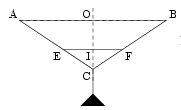
\includegraphics[scale=1]{RepS-47.png}
\end{multicols}
\begin{enumerate}
\item Quelle est la valeur exacte $\cal V$, en cm$^3$, du volume du
verre ?
\item Exprime, en fonction de $\pi$, le volume total de glace, en
cm$^3$.
\item Lors de la fusion de la glace, le volume de l'eau produite est
obtenu en multipliant par 0,9 celui de la glace. Quelle est la valeur
exacte $\cal W$, en cm$^3$, du volume d'eau dans le verre, résultant
de la fusion complète des cinq glaçons ?
\item Prouve que ${\cal V}=8{\cal W}$.
\item Déduis-en la hauteur $CI$ de l'eau dans le verre à pied après
fusion complète de la glace.
\end{enumerate}

